\documentclass[utf8, seminar]{fer}
\usepackage{booktabs}
\usepackage{hyperref}
\usepackage{siunitx}
\usepackage{amsmath}


\begin{document}

\title{Analiza periodičkih struktura s naglaskom na fotoničke kristale
	   i izračun disperzijskog dijagrama}
\author{Darko Janeković}
\voditelj{dr.sc. Dario Bojanjac}

\maketitle

\tableofcontents


\chapter{Uvod}
U ovom seminaru bit će riječi o analizi periodičkih struktura gdje će naglasak
biti na fotoničkim kristalima i primjeni numeričkih metoda na izračun
disperzijskog dijagrama. Programska biblioteka koja se koristi za numeričko
modeliranje je \href{https://github.com/stevengj/mpb}{MPB}. Prije svega, bit će
iznesena matematička podloga potrebna za efikasno modeliranje širenja vala u
periodičkoj strukturi. U poglavljima nakon uvoda bit će iznesena primjena
fotoničkih kristala, kao i numeričke metode korištene u svrhu modeliranja
problema koji opisuju periodičke strukture.


\chapter{Matematičko modeliranje širenja vala u periodičkoj strukturi}

%SADŽAJ POGLAVLJA: prvo napiši nešto o periodičkim strukturama/simetrija/rešetka
% Blochov teorem
% Valna za širenje vala u nehomogenom dielektriku
% Njena interpretacija, kako će se odnositi energija i slično
% Sve spoji u jedno i onda spomeni svojstveni problem kako se on rješava i da
% će sve dalje biti računato iz te jednadžbe

U ovom poglavlju nešto će detaljnije biti iznesena teorija periodičkih struktura
kao i matematički formalizam koji ih opisuje. Analiza propagacije vala unutar
periodičke rešetke prirodno navodi na Blochov teorem. On tvrdi da će polje u
periodičkoj strukturi poprimiti isti period i simetriju kao i period te strukture.
Kao polazišna točka bit će izvedena valna jednadžba za propagaciju vala unutar
nehomogenog dielektrika. Svojstveni problem i njegova interpretacija bit će
razmatrani baš u okvirima te jednadžbe. Konačno će jednadžba pomoću Blochovog
teorema biti specijalizirana za slučaj periodičke strukture.


\section{Periodičke strukture i kristalna rešetka}

Periodička struktura je pravilna struktura u kojoj se elementi na neki način
periodički ponavljaju. U nastavku će biti razmatrani fotonički kristali koji se
mogu razmatrati kao kristalne rešetke. Fotonički kristali su periodični na način
da zadovavaju diskretnu translacijsku simetriju.
Diskretna translacijska simetrija definirana je kao
${f(\mathbf{r}) = f(\mathbf{r} \pm \mathbf{a})}$, odnosno

\begin{equation}
	f(\mathbf{r}) = f(\mathbf{r} + \mathbf{R}) \text{, gdje je }{\mathbf{R} =
	n\mathbf{a}} \text{, a } n \in \mathbb{Z}
\end{equation}

Vektor $\mathbf{a}$ naziva se primitivni vektor rešetke, a njegova duljina
naziva se konstanta rešetke. Ćelija za koju se tvrdi da svojim ponavljanjem
tvori kristalnu rešetku naziva se jedinična ćelija. Jedinična ćelija je
najmanja jedinica kristalne rešetke koja svojim ponavljanjem može tvoriti
potpunu rešetku. Pored toga, ne postoji ćelija manjeg volumena od
${|\mathbf{a}_1 \cdot \mathbf{a}_2 \times \mathbf{a}_3|}$, odnosno volumena
kojeg zatvaraju primitivni vektori rešetke.

%NOTE: bilo bi zgodno da ovdje ubacim sliku kristalne rešetke sa svim ucrtanim vektorima

Ovisno o dimenzionalnosti problema moguće je odabrati različite primitivne
vektore rešetke i sve ostale translacije prikazati kao linearnu kombinaciju
primitivnih vektora.

Weigner-Seintzova ćelija primjer je primitivne ćelije koja sadrži samo jedno
čvorište i predstavlja skup točaka u prostoru koji je bliži jednom čvorištu
od bilo kojeg drugog čvorišta. Čvorišta kristalne rešetke nalaze se u središtu
Weigner-Seintzova ćelije. Iako kristal ima beskonačno puno jediničnih ćelija,
on ima samo jednu Weigner-Seintzovu ćeliju.

Recipročna rešetka uvodi se za prikaz valnih vektora u Fourierovom razvoju
periodičkih funkcija. Vektori recipročne rešetke bit će označavani s $\mathbf{b}$.
Za vektore recipročne rešetke vrijedi:

\begin{equation}
	\mathbf{R} \cdot \mathbf{G} =
	(n_1\mathbf{a}_1 + n_2\mathbf{a}_2 + n_3\mathbf{a}_3)
	\cdot
	(m_1\mathbf{b}_1 + m_2\mathbf{b}_2 + m_3\mathbf{b}_3) = 2 \pi \mathbb{N},
		\text{ gdje je }n_i, m_i \in \mathbb{Z}
\end{equation}


Weigner-Seintzova ćelija recipročne rešetke zove se Brillouinova zona. Analiza
disperzijskog dijagrama obavlja se u \textit{k prostoru} ili u prostoru
recipročne rešetke, odnosno u prvoj Brillouinovoj zoni. Prva Brillouinova zona je
najmanji prostor unutar Brillouinove zone koji u potpunosti karakterizira polje
unutar periodičke strukture. Svaku točku unutar Brillouinove zone moguće je
preslikati u prvu Brillouinovu zonu. Drugim riječima, analiza širenja vala unutar
Brillouinove zone, bit će ekvivalenta analizi unutar prve Brillouinove zone uz
određenu redundantnost u računu. Što je rešetka više simetrična, to će biti
isplativije analizu obavljati unutar prve Brillouinove zone.


\section{Blochov teorem}

Intuitivnim razmišljanjem jasno je da će val koji je u jednom trenutku prolazio
kroz dielektrični objekt kasniti u odnosu na val koji nije. Lako je onda
generalizirati ideju na periodičku strukturu i iz tog razmišljanja izvući
zaključak da će polje unutar periodičke strukture poprimiti isti period i
simetriju kao i ta struktura. Teorem koji je upravo intuitivno izveden naziva se
Blochov teorem, i matematički formaliziran glasi ovako:

\begin{equation} \label{eq:bloch}
	\mathbf{E}(\mathbf{r}) =
	\mathbf{A}(\mathbf{r}) \cdot e^{j \mathbf{\beta} \cdot \mathbf{r}}
\end{equation}

U jednadžbi \ref{eq:bloch}, vektorsko polje $\mathbf{E}$ označava ukupno polje
u periodičkoj strukturi i ono se sastoji od dvije komponente. Vektorsko polje
$\mathbf{A}$ označava envelopu s istim periodom i simetrijom kao i rešetka.
Ono diktira amplitudu ukupnog polja $\mathbf{E}$.
Komponenta ${e^{j \mathbf{\beta} \cdot \mathbf{r}}}$ označava ravni val i diktira
smjer širenja vala.

% ubaci meep sliku kako to izgleda i napiši par riječi o tome

% matematički potkrijepi gore napisano + pročitaj više o ovome


\section{Izvod valne jednadžbe za širenje u sredstvu s nehomogenim dielektrikom}

U ovom potpoglavlju bit će izvedena valna jednadžba koja opisuje propagaciju
vala u nehomogenom dielektriku. Sredstvo u kojem val propagira nalikuje sredstvu
na slici.

% TODO: label i uredi sliku
\begin{figure}
	\centering
	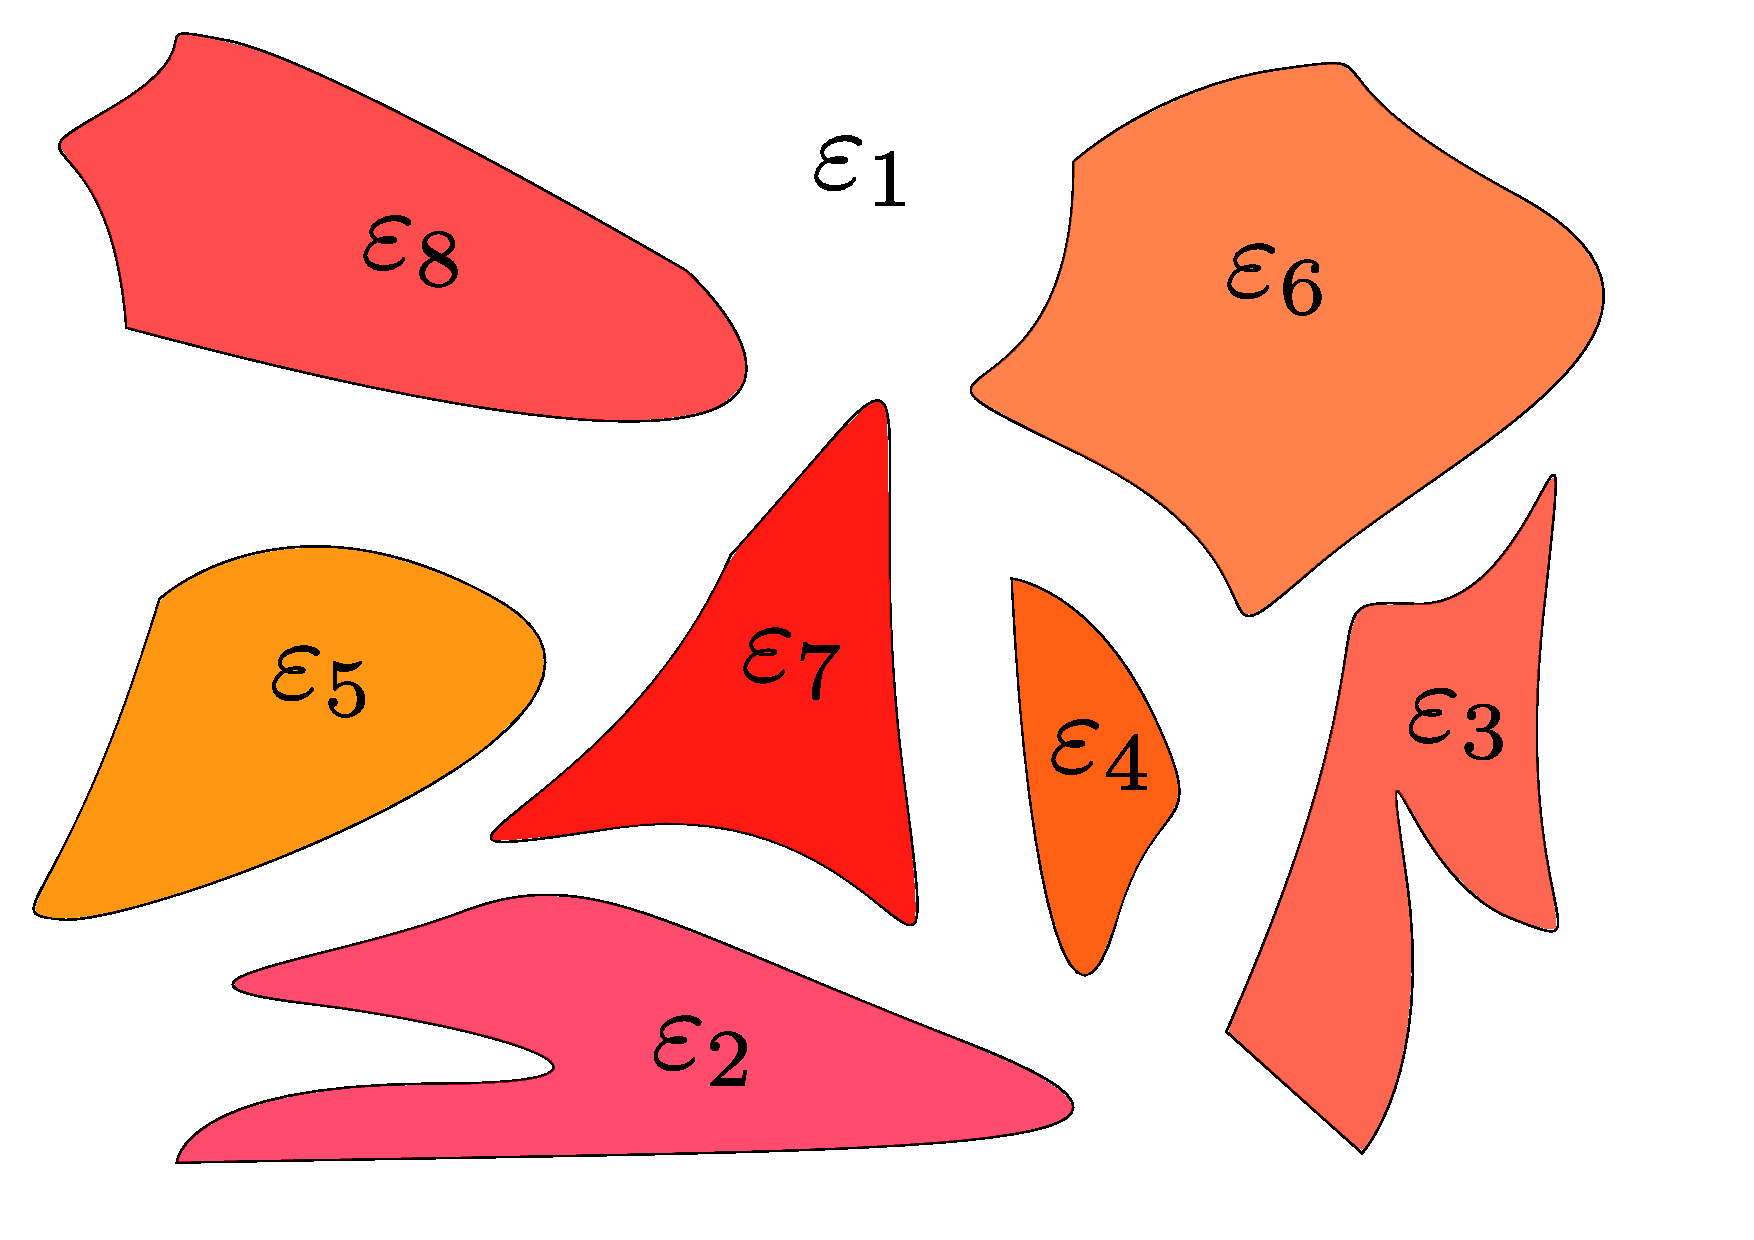
\includegraphics[scale=0.5]{./images/structure-model.pdf}
\end{figure}

Izvod valne jednadžbe, kao i za slučaj propagacije u homogenom sredstvu počinje
s Maxwellovim jednadžbama:

\begin{align} \label{eq:maxwell1}
	\nabla \cdot \mathbf{D} = \rho &&
	\nabla \times \mathbf{E} &=
		- \frac{\partial \mathbf{B}}{\partial t}  \nonumber \\
	\nabla \cdot \mathbf{B} = 0 &&
	\nabla \times \mathbf{H} &=
		\mathbf{J} + \frac{\partial \mathbf{D}}{\partial t}
\end{align}

$\varepsilon$ u sredstvu postaje funkcija koja ovisi o položaju, odnosno
$\varepsilon(\mathbf{r})$. Pored toga, pretpostavlja se da struktura ne mijenja
konfiguraciju u vremenu, te da u njoj nema izvora svjetlosti. Između ostalog
pretpostavlja se da su snage dovoljno male kako bi sustav imalo smisla promatrati
u linearnom režimu.
% NOTE: napiši što se koristi u protivnom, Bloembergen suma (2)
Materijal u kojem se vrši propagacija promatra se kao izotropan na makroskopskoj
razini. U slučaju anizotropnog medija $\mathbf{D}$ i $\mathbf{E}$ nisu vezani
s $\varepsilon_0 \varepsilon$, već s
%TODO: potkrijepi citatom iz dario knjige + pročitaj više
dielektričnim tenzorom $\varepsilon_0 \varepsilon_{ij}$. Frekvencijska
ovisnost dielektrične permeabilnosti bit će zanemarena. Konačno, nakon svih
pretpostavki jednadžbe \ref{eq:maxwell1} poprimaju sljedeći oblik:

\begin{align} \label{eq:maxwell2}
	\nabla \cdot (\varepsilon(\mathbf{r}) \mathbf{E}(\mathbf{r}, t)) = 0 &&
	\nabla \times \mathbf{E}(\mathbf{r}, t) &=
		- \mu_0 \mu(\mathbf{r})
		\frac{\partial \mathbf{H}(\mathbf{r}, t)}{\partial t}  \nonumber \\
	\nabla \cdot \mathbf{H}(\mathbf{r}, t) = 0 &&
	\nabla \times \mathbf{H}(\mathbf{r}, t) &=
		\varepsilon_0 \varepsilon(\mathbf{r}, t)
		\frac{\partial \mathbf{E}(\mathbf{r}, t)}{\partial t}
\end{align}

Budući da su Maxwellove jednadžbe linearne, moguće je pretpostaviti da će pobuda
titrati istom frekvencijom kao i pobuda. To svojstvo omogućava rastav polja
na prostornu i vremensku komponentu. Rastav se obavlja preko sljedećeg zapisa:
% TODO: citat dario knjiga
% napiši i pročitaj više o ovome
\begin{equation} \label{eq:harmonic}
	\mathbf{H}(\mathbf{r}, t) = \mathbf{H}(\mathbf{r}) e^{-i \omega t}
\end{equation}

Nakon uvrštavanja \ref{eq:harmonic} Maxwellove jednadžbe poprimaju sljedeći
oblik:

\begin{align} \label{eq:maxwell3}
	\nabla \cdot (\varepsilon(\mathbf{r}) \mathbf{E}(\mathbf{r})) = 0 &&
	\nabla \times \mathbf{E}(\mathbf{r}) &=
		i \omega \mu_0 \mu(\mathbf{r})\mathbf{H}(\mathbf{r})  \nonumber \\
	\nabla \cdot \mathbf{H}(\mathbf{r}) = 0 &&
	\nabla \times \mathbf{H}(\mathbf{r}) &=
		- i \omega \varepsilon_0 \varepsilon(\mathbf{r})\mathbf{E}(\mathbf{r})
\end{align}

Djelujući rotorom na jednadžbu koja opisuje Faradayev zakon dobiva se valna
jednadžba u sljedećem obliku:

\begin{equation} \label{eq:master}
	\nabla \times \left(\frac{1}{\varepsilon(\mathbf{r})}\nabla
			\times \mathbf{H}(\mathbf{r}) \right)
			= \left( \frac{\omega}{c} \right)^2 \mathbf{H}(\mathbf{r})
\end{equation}

Jednadžba \ref{eq:master} predstavljat će jednadžbu koja će biti korištena za
računanje disperzijskog dijagrama za propagaciju vala u nehomogenom dielektriku.
Ako se ${\nabla \times \frac{1}{\varepsilon(\mathbf{r})} \nabla \times}$
zamijeni s $\hat{\mathbf{\Theta}}$ dobiva se uobičajena forma svojstvenog
problema.

\begin{equation}
	\hat{\mathbf{\Theta}} \mathbf{H}(\mathbf{r}) =
		\left( \frac{\omega}{c} \right)^2 \mathbf{H}(\mathbf{r})
\end{equation}

Budući da je operator $\hat{\mathbf{\Theta}}$ hermitski\footnote{napiši dokaz u
kratkim crtama}


% napiši o svojstvima koja se daju izvaditi iz ovog, energije i slično i onda sve
% spoji s blochovim teoremom tako da je i periočka rešetka pokrivena


\chapter{Zaključak}
Zaključak.

\bibliography{literatura}
\bibliographystyle{fer}

\chapter{Sažetak}
Sažetak.

\end{document}
